\documentclass[12pt, a4paper]{article}
\usepackage[T1]{fontenc}
\usepackage[utf8]{inputenc}
\usepackage[french]{babel}
\usepackage{geometry}
\usepackage{graphicx}
\usepackage{wrapfig}
\usepackage{indentfirst}

\graphicspath{{/home/pgi/TIPE/content/Rapport/image/}}

% Title
\title{Rapport de TIPE\\
Morpion}
\author{Peng-Wei Chen, MP, \oldstylenums{2017}-\oldstylenums{2018}}

\begin{document}

\maketitle

\section{Introduction}
\subsection*{La règle du morpion}
Deux joueurs jouent sur une grille de taille $15 \times 15$ sur le papier. Chaqu'un prend un symbole et on dessine au tour par tour son symbole sur la grille. Le but est d'aligner 5 symboles verticalement, horizontalement ou en diagonale pour gagner.
Dans le cas généralisé, nous appelons (m, n, k)-jeu où la taille de la grille est $m \times n$ et il faut $k$ symboles dans une ligne pour gagner.
\subsection*{Méthode}
Il existe deux méthodes pour déterminer s'il existe une telle stratégie:
\begin{itemize}
    \item On cherche tous les cas possibles.
    \item On apparie les points de la grille. Si le deuxième joueur peut toujours prévenir la réussite du premier joueur en jouant le pairage, alors il n'y a pas d'une telle stratégie.
\end{itemize}

Dans le cas où k $\le$ 7, on utilise la première méthode avec l'arbre de décision. Chaque nœud de cet arbre est un état de la grille. Par exemple (figure. \ref{fig:arbre}) , la racine de cet arbre est la grille sans symbole. Ensuite, les fils de chaque nœud sont les états de la grille où on place un symbole de plus au dessus. Enfin, les feuilles sont les cas où un des joueurs a gagné ou où personne n'a gagné (c'est-à-dire que la grille a été remplie et que aucun joueur a aligné k symboles).

\begin{figure}[t]
\centering
\includegraphics[height=6cm]{arbre.eps}
\caption{Arbre de décision (le cercle noir est le symbole du premier joueur)} \label{fig:arbre}
\end{figure}

Or, la complexité de chercher tous les cas possibles est en O(($m \times n$)!). Ainsi, on utilise une fonction gloutonne pour chercher le cas le \og plus \fg possible. Avec cette fonction, on donne une note à chaque point. Si un point est plus possible pour gagner, alors sa note est plus élevée.
\\
On utilise la deuxième méthode lorsque k > 7.

\section{Exploitation}
\subsection*{k $\le$ 5}
%% alpha-beta

\subsection*{k $\ge$ 8}
En effet, si on peut montrer que le premier joueur n'a pas de stratégie gagnante lorsque k = 8, alors le premier joueur n'en a pas pour tout k $\ge$ 8 car la même stratégie du deuxième joueur parvient le premier à aligner 8 symboles.
On donne notamment le pairage du cas k = 9 (figure. \ref{fig:m-n-9}) car il est plus intuitif.
\begin{figure}[h!]
    \centering
    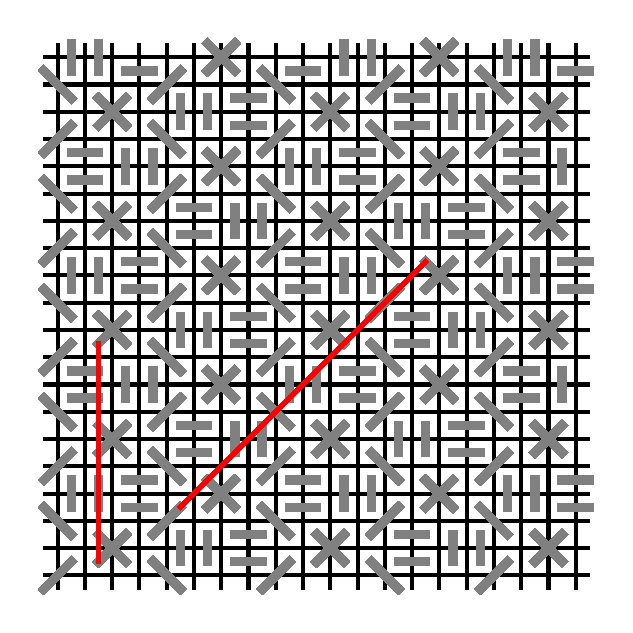
\includegraphics{m-n-9.eps}
    \caption{(m, n, 9)-jeu}
    \label{fig:m-n-9}
\end{figure}
On voit que si le deuxième joueur suit le pairage, alors le premier joueur ne peut jamais réussir (les lignes rouges).\\
Lorsque k = 8, on divise le jeu en des sous-jeux. Ces sous-jeux se jouent sur la grille de la forme comme \mbox{figure. \ref{fig:sous-jeu}.}
\begin{figure}[h!]
    \centering
    \includegraphics{m-n-8-little.eps}
    \caption{La grille du sous-jeu}
    \label{fig:sous-jeu}
\end{figure}
Il y a trois façons de gagner ce sous-jeu \mbox{(figure. \ref{fig:regle}):}
\begin{itemize}
    \item Aligner trois symboles en diagonale.
    \item Aligner verticalement deux symboles.
    \item Aligner horizontalement quatre symboles.
\end{itemize}
\begin{figure}[h!]
    \centering
    \includegraphics{8-rules1.eps}
    \includegraphics{8-rules2.eps}
    \includegraphics{8-rules3.eps}
    \caption{Les trois façons pour gagner dans le sous-jeu.}
    \label{fig:regle}
\end{figure}
Ainsi, puisque le premièr joueur ne peut jamais gagner ce sous-jeu, il ne peut pas non plus gagner le (m, n, 8)-jeu. (figure. \ref{fig:m-n-8})
\begin{figure}[h!]
    \centering
    \includegraphics{8-sol.eps}
    \caption{(m, n, 8)-jeu:
    toutes les lignes de longueur 8 passent une des lignes du sous-jeu.}
    \label{fig:m-n-8}
\end{figure}
\section{Conclusion}

\begin{itemize}
    \item k = 1
    \item k = 2
    \item k = 3
    \item k = 4
    \item k = 5
    \item k $\ge$ 8\\
        Une telle stratégie n'existe pas.
\end{itemize}


\end{document}
